\chapter{Models and Documentation}\label{ch:listings}
%% use language 'myLng' for the next listings (until another language is set)
%% include listing 'listings/AdverseReactionApp.aj' with label and caption
%% note: big listings sometimes need to overwrite the float value that has been
%% already set in the general listings setup (see paper.tex)

% This chapter contains the beautiful listing \ref{lst:system}. 

In this section, we present the models developed for the hospital information system using Monticore, a domain-specific modeling language and toolset, as well as Business Process Model and Notation (BPMN) diagrams. The models serve as visual representations of the system's structure, behavior, and interactions, offering stakeholders a comprehensive understanding of the various components and functionalities of the hospital information system.

\section{Class Diagrams}

% \begin{landscape}
\begin{figure}[htbp]
  \centering
  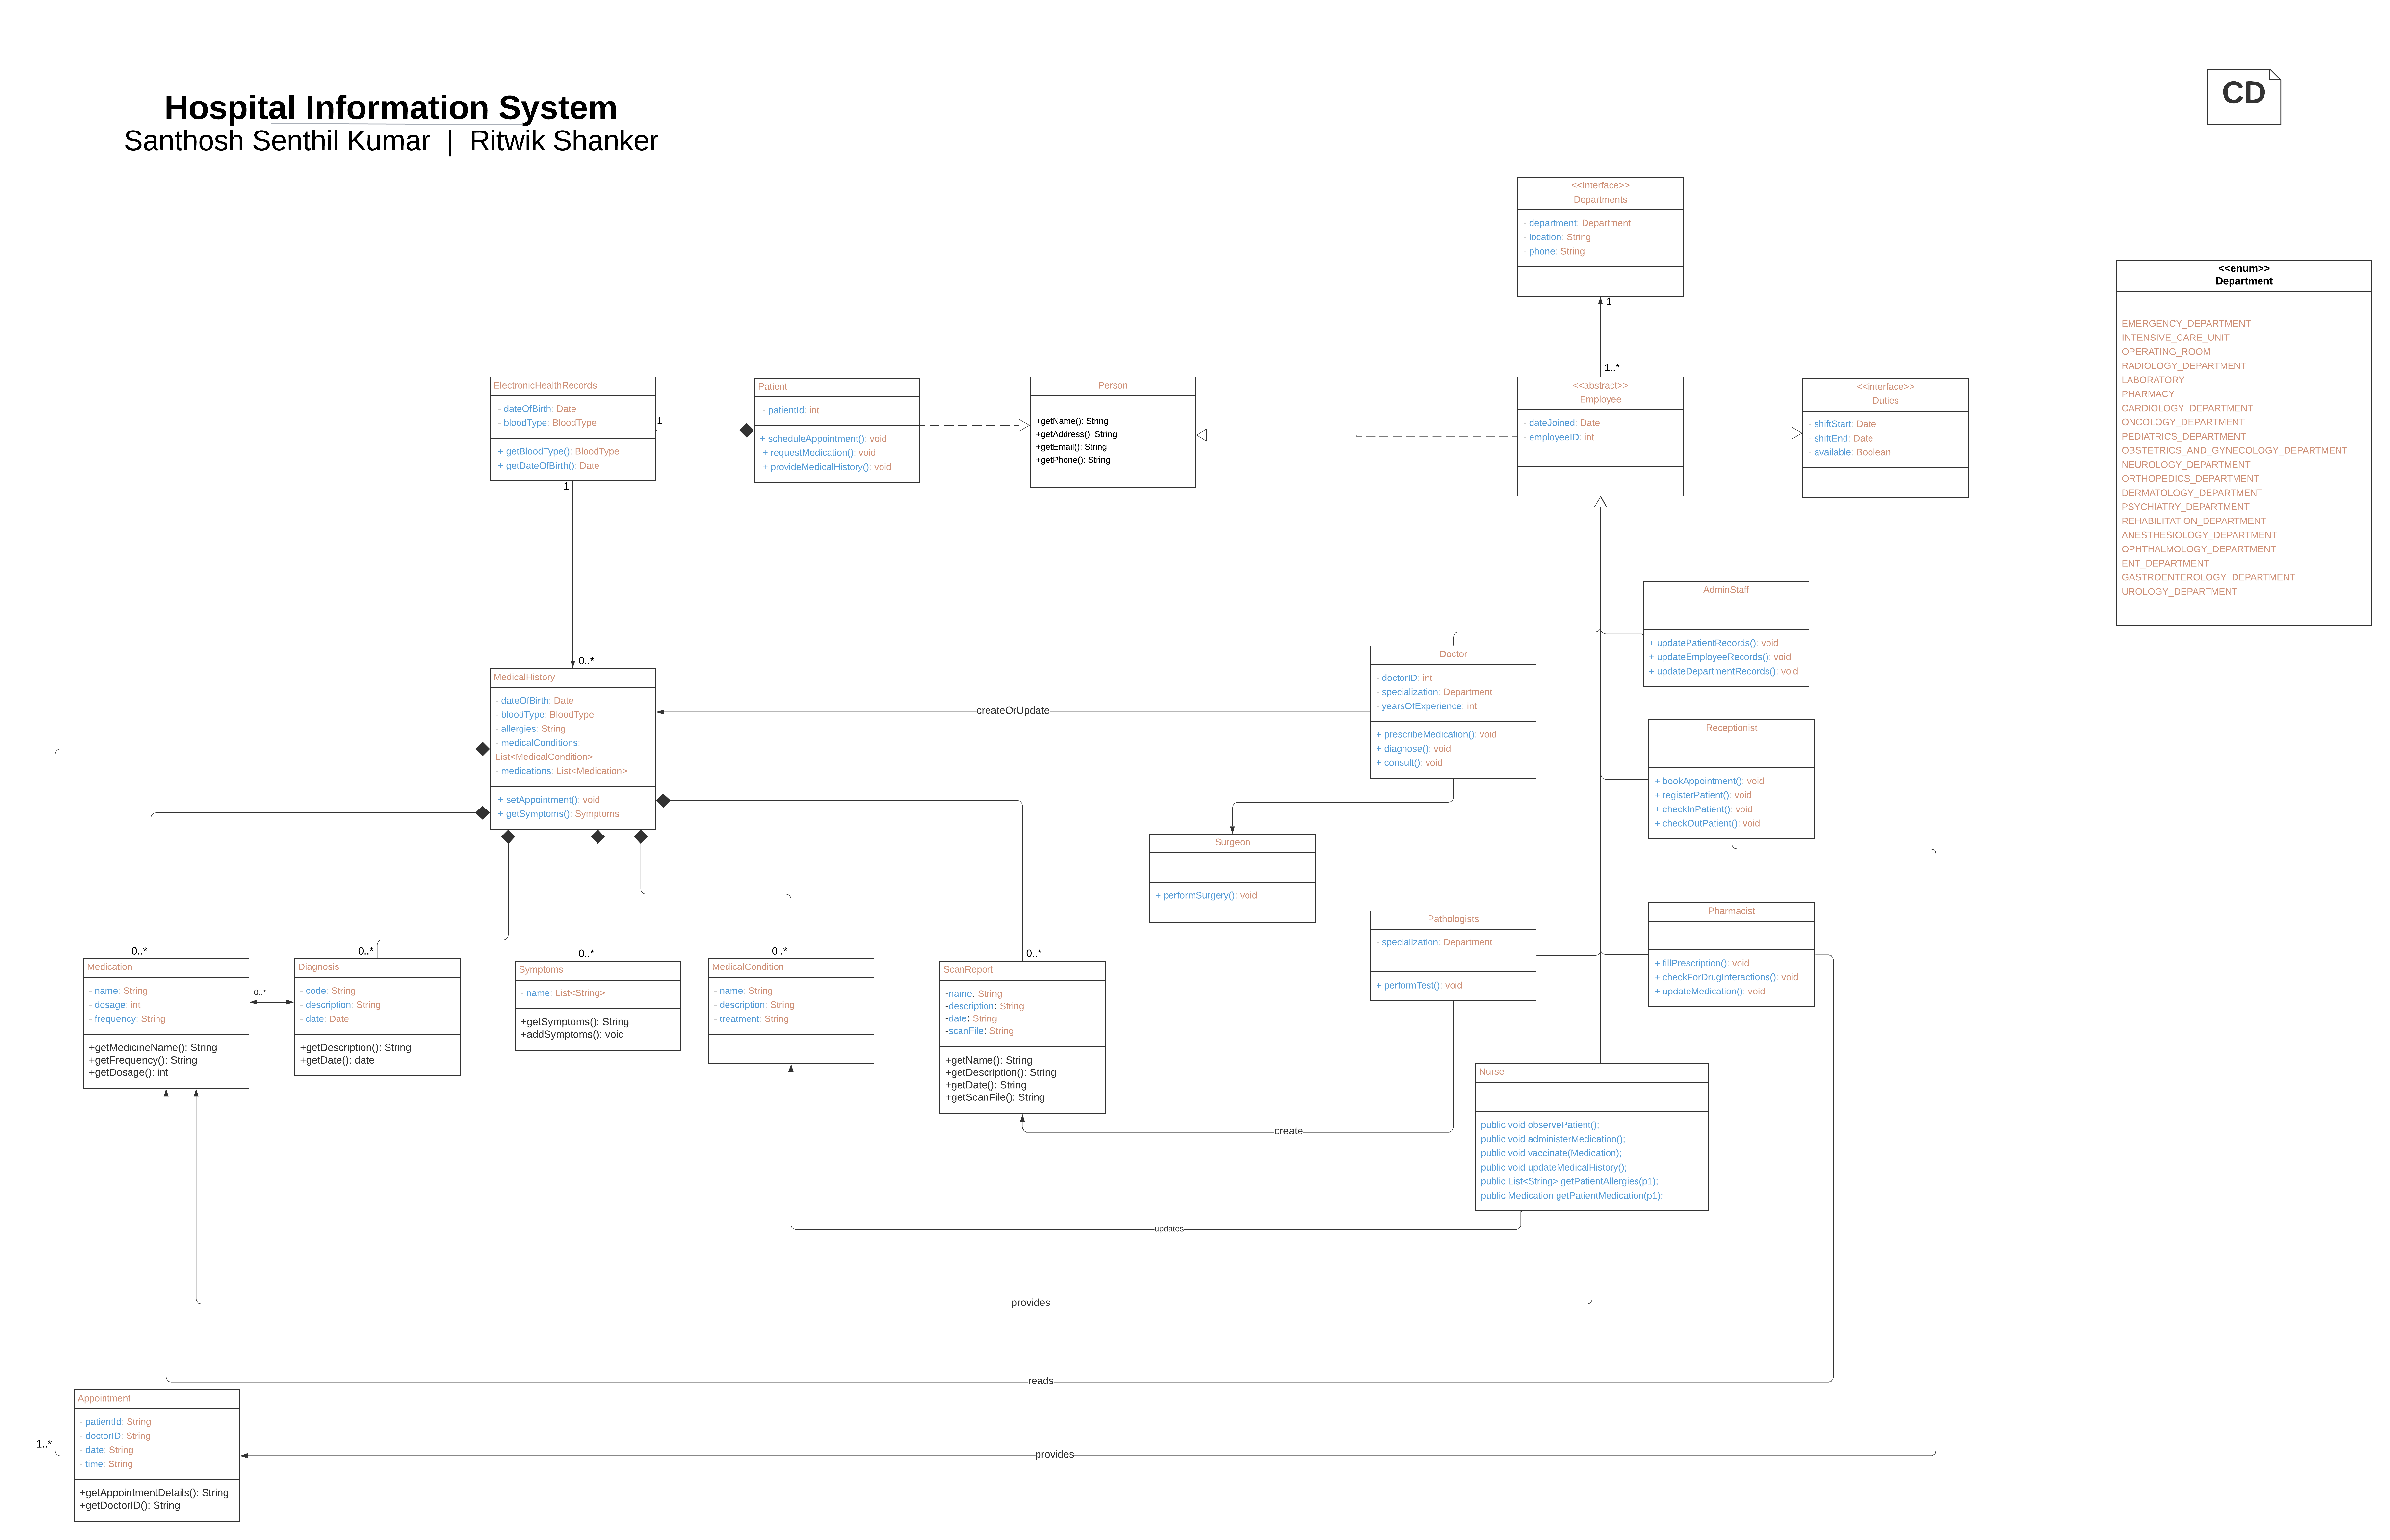
\includegraphics[width=\textwidth,height=\textheight,keepaspectratio]{src/pic/UML class.png}
  \caption{Visual Representation of Class Diagram showing all the classes}
  \label{fig:fullscreen}
\end{figure}
% \end{landscape}



\subsection{Patient}
\begin{figure}[hbt]
\lstset{language=MontiArc}
\lstinputlisting[
label=lst:patientcd,
caption=Class Diagram for Patient Class] {src/listings/CD/Patient.cd}
\end{figure}

The \texttt{Patient} class represents a patient in a healthcare system. It extends the \texttt{Person} class and adds additional attributes specific to patients. The \texttt{Person} class contains common attributes such as ID, name, address, email, and phone.

The \texttt{Patient} class has the following operations:
\begin{itemize}
  \item \texttt{scheduleAppointment()}: Allows the patient to schedule an appointment.
  \item \texttt{requestMedication()}: Allows the patient to request medication.
  \item \texttt{provideMedicalHistory()}: Allows the patient to provide their medical history.
\end{itemize}

The \texttt{Patient} class has a composition relationship with the \texttt{MedicalHistory} class, indicating that each patient has a medical history. This relationship is denoted by the arrow connecting \texttt{Patient} to \texttt{MedicalHistory} with a multiplicity of \texttt{[*]}, meaning each patient can have multiple medical history records.

\subsection{Hospital}
\lstinputlisting[language=MontiArc,breaklines=true,caption=Class Diagram for Hospital Class]{src/listings/CD/Hospital.cd}

% \begin{figure}[hbt]
% \lstset{language=MontiArc}
% \lstinputlisting[
% label=lst:hospcd,
% caption=Class Diagram for Hospital Class] {src/listings/CD/Hospital.cd}
% \end{figure}

The \texttt{Hospital} class has the following nested classes:
\begin{itemize}
  \item \texttt{Departments}: Represents a department in the hospital. It has attributes such as the department name, location, and phone number.
  \item \texttt{Receptionist}, \texttt{Nurse}, \texttt{Pharmacist}, \texttt{AdminStaff}, \texttt{Pathologists}, \texttt{Doctor}, and \texttt{Surgeon}: These classes represent different types of employees in the hospital. They extend the \texttt{Employee} class, which itself extends the \texttt{Person} class. Each employee class has specific operations related to their role in the hospital.
\end{itemize}


The \texttt{Hospital} class also has an enumeration called \texttt{Department}, which lists various departments in the hospital.

There are associations between the classes:
\begin{itemize}
  \item \texttt{Employee} has a composition relationship with \texttt{Duties}, indicating that each employee has one or more duties.
  \item \texttt{AdminStaff} has a supervision relationship with other employees, denoted by the association between \texttt{AdminStaff} and \texttt{Employee}.
  \item \texttt{Doctor} has a relationship with \texttt{Departments}, indicating that each doctor can head a department, and each department can have a head doctor.
  \item \texttt{Employee} has a relationship with \texttt{Departments}, indicating that each employee works in one department.
\end{itemize}

\subsection{Electronic Health Record}

\lstinputlisting[language=MontiArc,breaklines=true,caption=Class Diagram for EHR Class]{src/listings/CD/EHR.cd}
% \begin{figure}[hbt]
% \lstset{language=MontiArc}
% \lstinputlisting[
% label=lst:ehrcd,
% caption=Class Diagram for EHR Class] {src/listings/CD/EHR.cd}
% \end{figure}

The \texttt{EHR} class represents an Electronic Health Record (EHR) system. It contains several classes related to medical information.

The \texttt{EHR} class has the following nested classes:
\begin{itemize}
  \item \texttt{Symptoms}: Represents a list of symptoms.
  \item \texttt{Diagnosis}: Represents a medical diagnosis with attributes such as code, description, date, and associated symptoms.
  \item \texttt{ScanReport}: Represents a scan report with attributes such as name, description, date, and the file containing the scan.
  \item \texttt{Appointment}: Represents a scheduled appointment with attributes such as patient ID, doctor ID, date, and time.


  \item \texttt{Medication}: Represents a medication with attributes such as name, dosage, and frequency.
  \item \texttt{MedicalCondition}: Represents a medical condition with attributes such as name, description, and treatment. The treatment attribute within the MedicalCondition class allows for the inclusion of information related to the recommended or prescribed procedures, medications, therapies, or lifestyle modifications that are commonly associated with managing or treating that specific medical condition.
\end{itemize}

The \texttt{MedicalHistory} class is an abstract class representing the medical history of a patient. It contains attributes and relationships to various medical components such as allergies, medical conditions, medications, diagnoses, symptoms, scan reports, and appointments.

There are composition relationships between \texttt{MedicalHistory} and each of the medical components, indicating that a medical history consists of multiple instances of these components.

The \texttt{ElectronicHealthRecord} class represents an electronic health record for a patient. It contains attributes such as date of birth and blood type. It has a composition relationship with \texttt{MedicalHistory}, indicating that an electronic health record includes a patient's medical history.


\section{Sequence Diagrams}


\subsection{Patient Scan}

\begin{figure}[]
\lstset{language=MontiArc}
\lstinputlisting[
label=lst:pssd,
caption=Sequence Diagram for patient getting scanned] {src/listings/SD/patient-scan.sd}
\end{figure}

\begin{figure}[htb]
\begin{center}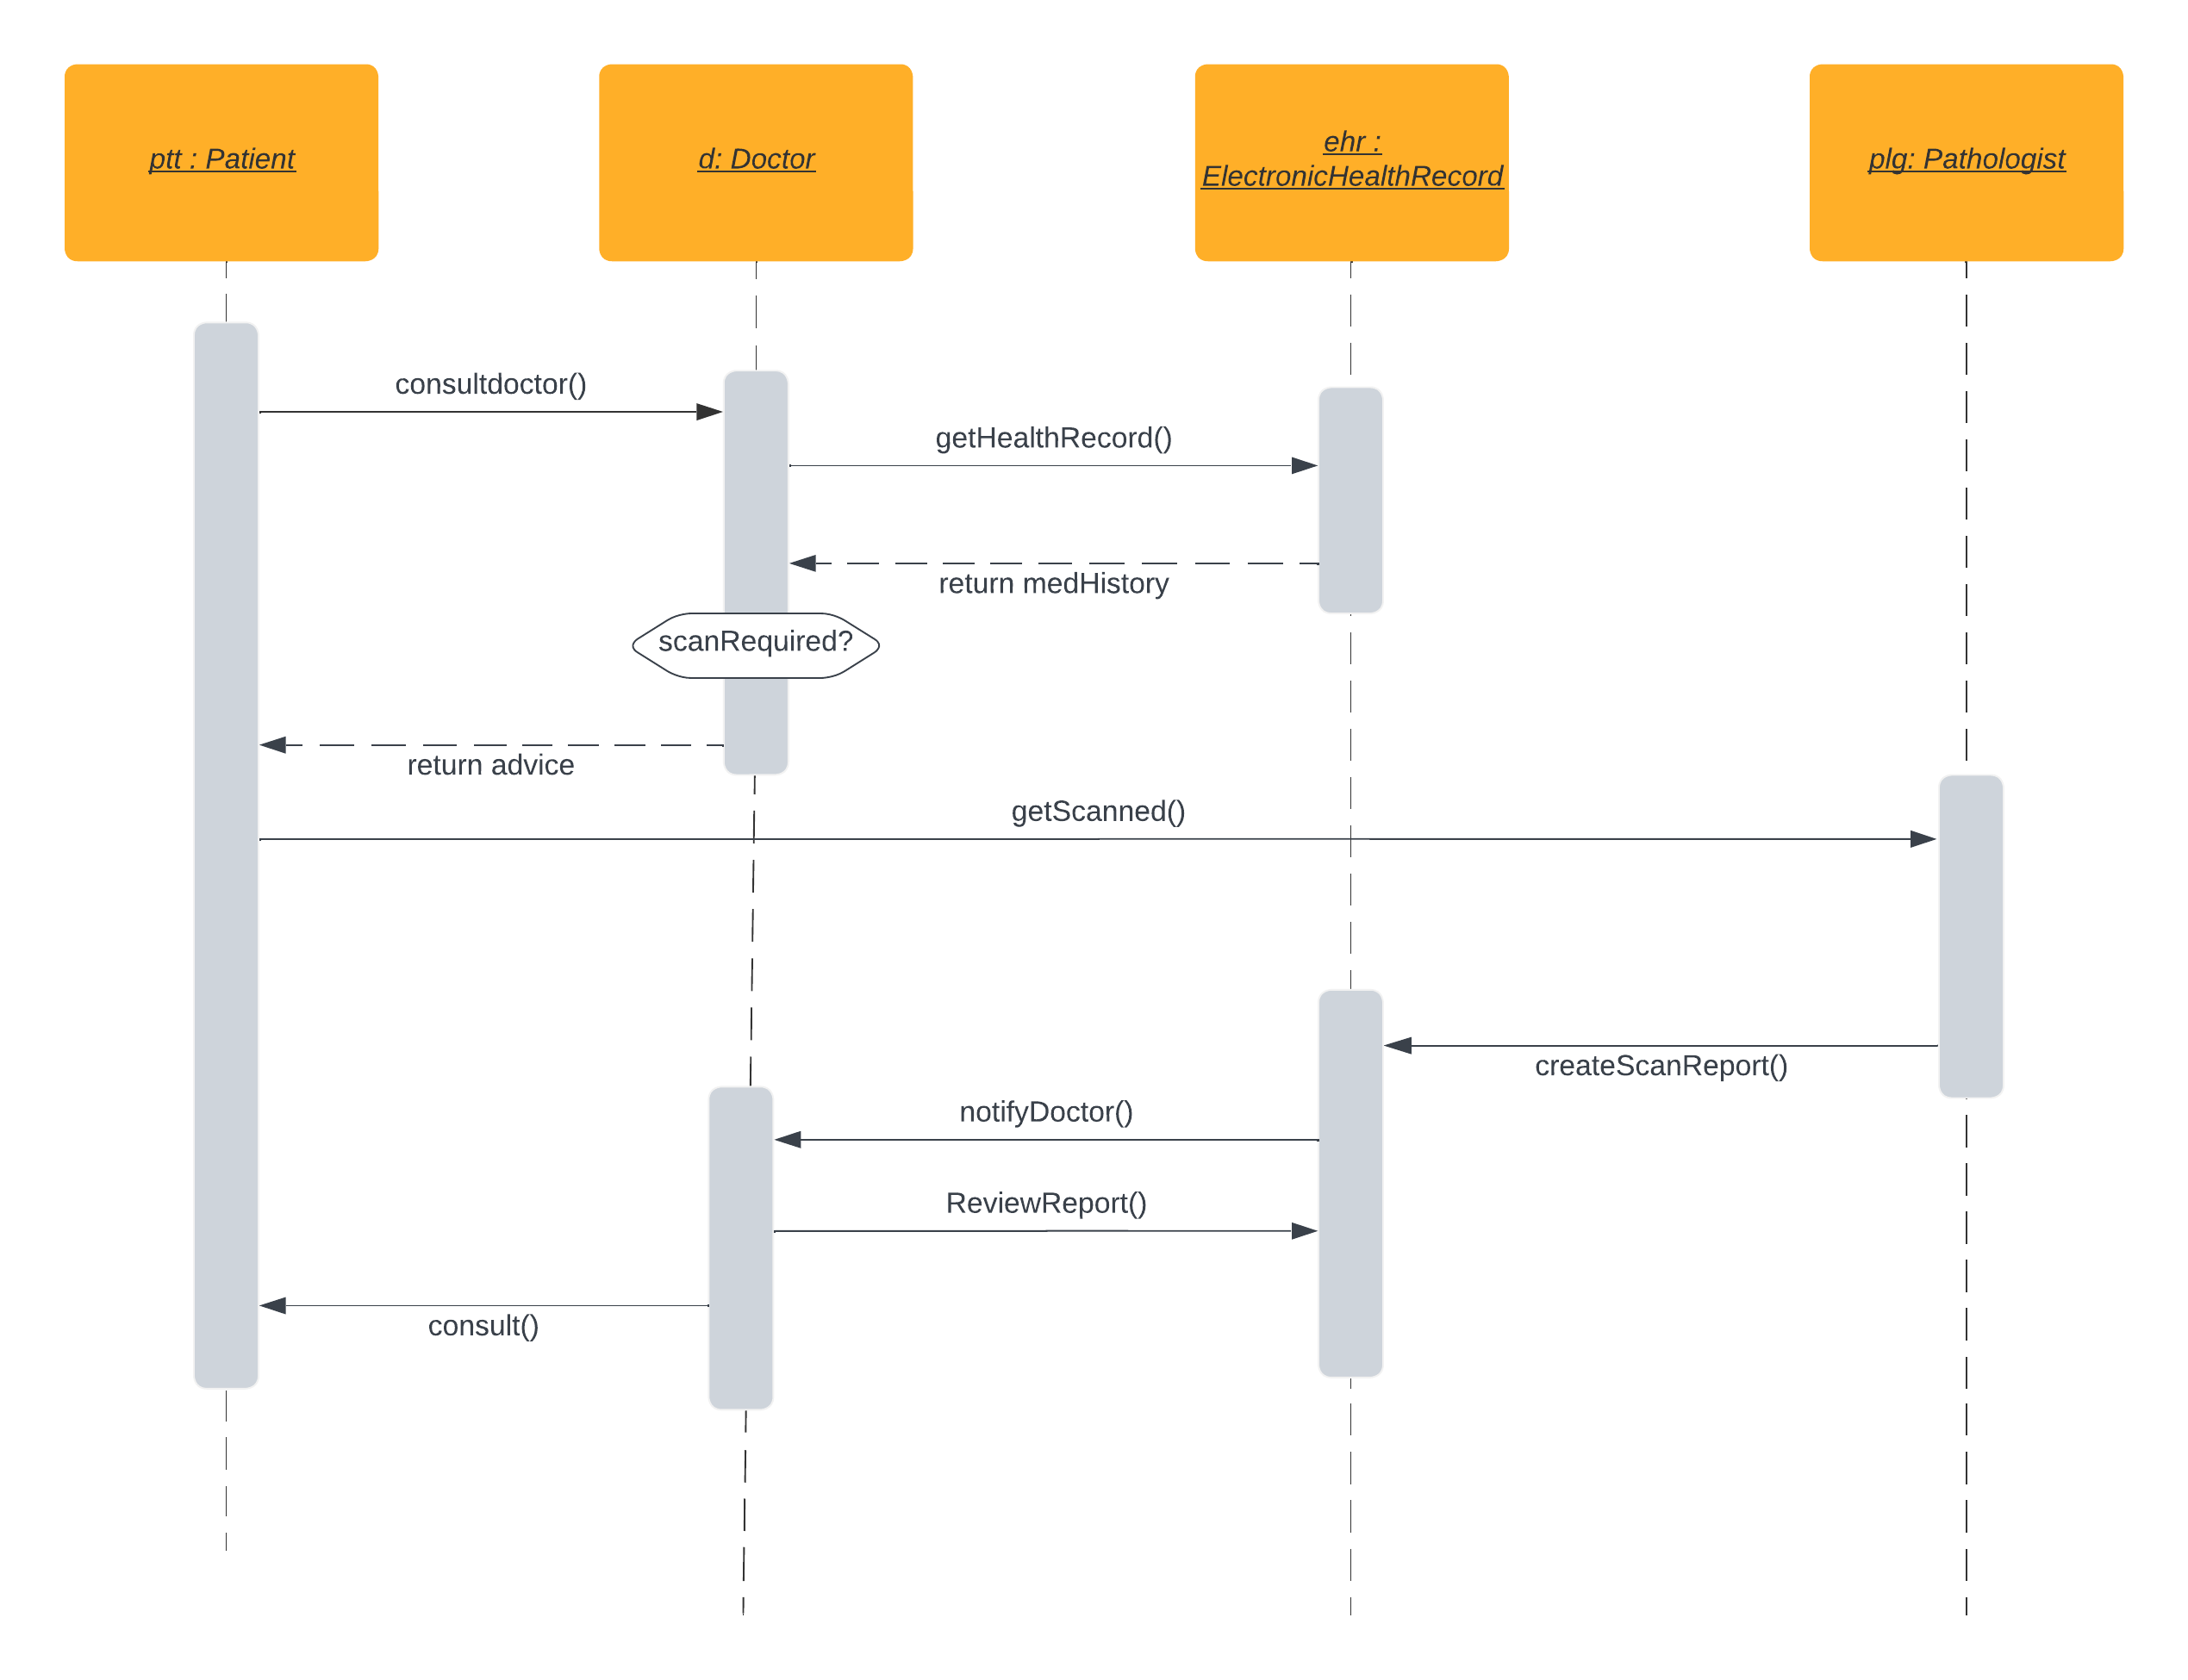
\includegraphics[width=12cm]{src/pic/SD1.png}\end{center}
\caption{Visual Sequence Diagram for Patient Scan process}
\label{SD1}
\end{figure}

The sequence diagram illustrates the interaction between a patient (\texttt{pt}), a doctor (\texttt{d}), an electronic health record (\texttt{ehr}), and a pathologist (\texttt{plg}) during a scanning process.

\begin{enumerate}
\item The patient initiates the \texttt{consultdoctor()} operation with the doctor.
\item The doctor retrieves the patient's health record from the electronic health record (\texttt{ehr}) using the \texttt{getHealthRecord(pt)} operation.
\item The electronic health record returns the medical history (\texttt{medHistory}) to the doctor.
\item The doctor verifies if a scan is required by checking the \texttt{scanRequired} attribute of the medical history. If it is true, the process continues; otherwise, the doctor provides advice to the patient and the sequence ends.
\item The doctor informs the patient of their advice using the \texttt{return advice} operation.
\item The patient requests the pathologist (\texttt{plg}) to get scanned by invoking the \texttt{getScanned()} operation.
\item The pathologist creates a scan report (\texttt{scanReport}) and sends it to the electronic health record using the \texttt{createScanReport(scanReport)} operation.
\item The electronic health record receives the scan report and acknowledges the pathologist.
\item The electronic health record notifies the doctor about the scan report using the \texttt{notifyDoctor(scanReport)} operation.
\item The doctor reviews the scan report using the \texttt{reviewReport()} operation.
\item The doctor consults with the patient using the \texttt{consult()} operation.
\item The patient responds to the doctor's consultation.
\item The doctor updates the medical history in the electronic health record using the \texttt{addHistory()} operation.
\end{enumerate}

\subsection{Vaccination}

The sequence diagram depicts the interaction between a patient (\texttt{p1}), a nurse (\texttt{nu1}), and an electronic health record (\texttt{ehr}) during a vaccination process that involves checking for allergies and using anti allergant along with the vaccine. This has been broken down into two parts, one for patient without allergies and one for with allergies.


\subsubsection{Vaccination of patient without allergies}
% \lstinputlisting[language=MontiArc,breaklines=true,caption=Class Diagram for EHR Class]{src/listings/CD/EHR.cd}




The sequence of events is as follows:

\begin{enumerate}
\item The patient arrives at the hospital and initiates the \texttt{arriveToHospital()} operation with the nurse.
\item The nurse retrieves the patient's allergies from the electronic health record using the \texttt{getAllergies(p1)} operation.
\item The electronic health record returns no allergies to the nurse.
\item The nurse administers the vaccination to the patient.
\item The nurse observes the patient and initiates the \texttt{ObservePatient()} operation.
\item The nurse updates the patient's medical history in the electronic health record using the \texttt{UpdateMedicalHistory()} operation.
\item The patient responds to the nurse's observation.
\end{enumerate}

\lstinputlisting[
label=lst:vpsd,
language=MontiArc,breaklines=true,
caption=Sequence Diagram for patient getting vaccinated without allergies] {src/listings/SD/vaccination.sd}

\begin{figure}[]
\begin{center}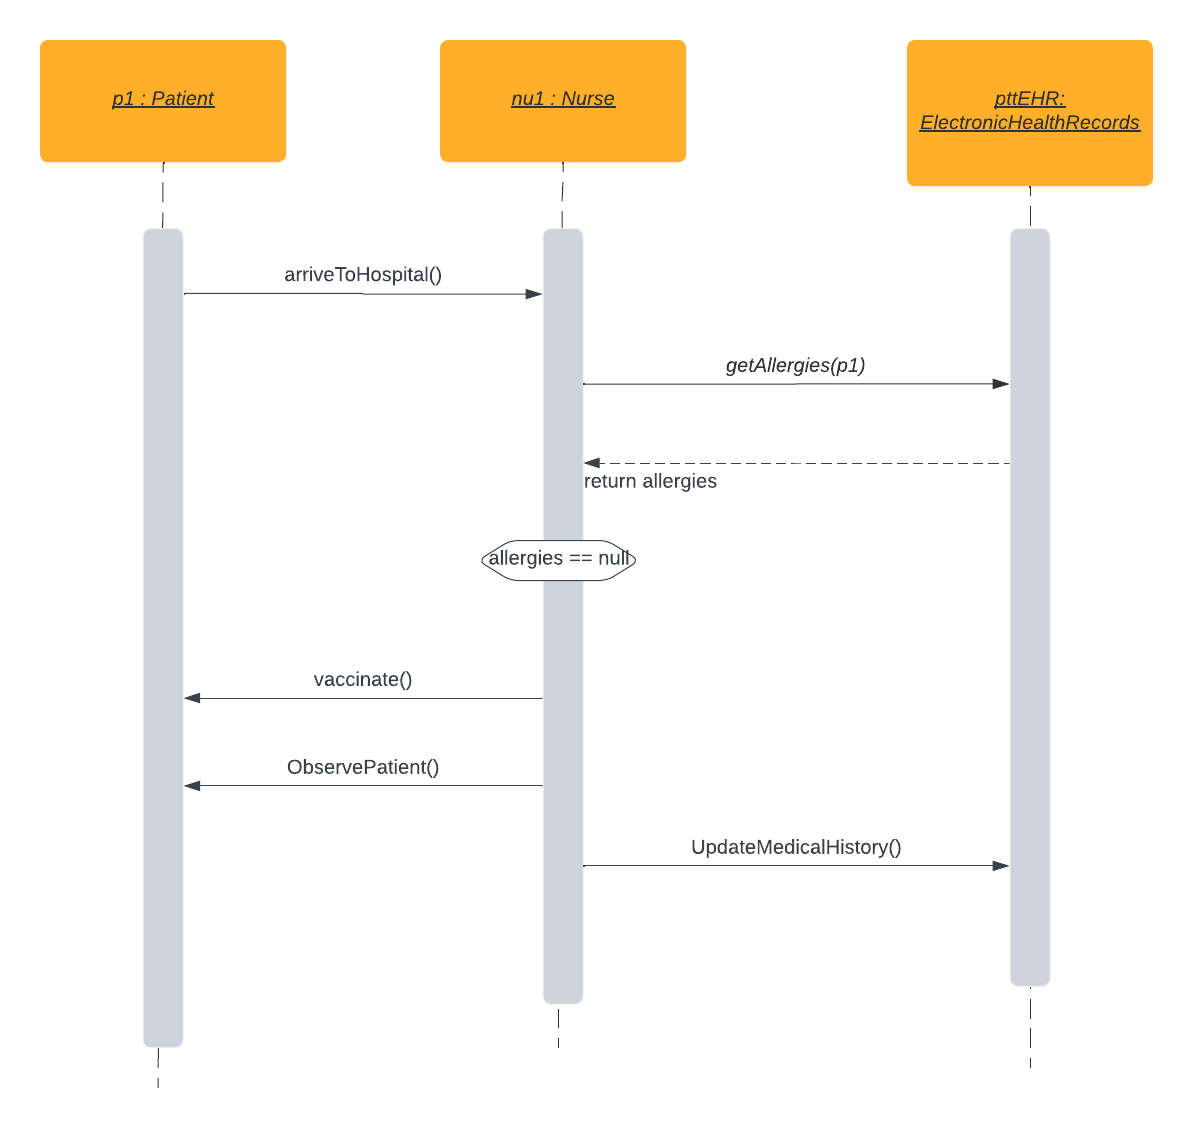
\includegraphics[width=12cm, height = 9cm]{src/pic/Vaccination_Without_Allergies.png}\end{center}
\caption{Visual Sequence Diagram for Vaccination of a Patient without Allergies}
\label{VAC1}
\end{figure}

\subsubsection{Vaccination of patient with allergies}

\begin{figure}[hbt]
\lstset{language=MontiArc}
\lstinputlisting[
label=lst:vpasd,
caption=Sequence Diagram for patient getting vaccinated without allergies] {src/listings/SD/vaccination-allergies.sd}
\end{figure}

\begin{enumerate}
\item The patient arrives at the hospital and initiates the \texttt{arriveToHospital()} operation with the nurse.
\item The nurse retrieves the patient's allergies from the electronic health record using the \texttt{getAllergies(p1)} operation.
\item The electronic health record returns the allergies to the nurse.
\item The nurse retrieves the patient's medication history (\texttt{mc1}) from the electronic health record using the \texttt{getMedication(p1)} operation.
\item The electronic health record returns the medication history to the nurse.
\item The nurse checks for an anti-allergen (\texttt{antiAllergent}) based on the medication history.
\item The nurse administers the vaccination to the patient, taking into account the anti-allergen.
\item The nurse observes the patient and initiates the \texttt{ObservePatient()} operation.
\item The nurse updates the patient's medical history in the electronic health record using the \texttt{UpdateMedicalHistory()} operation.
\item The patient responds to the nurse's observation.
\end{enumerate}

\begin{figure}[htb]
\begin{center}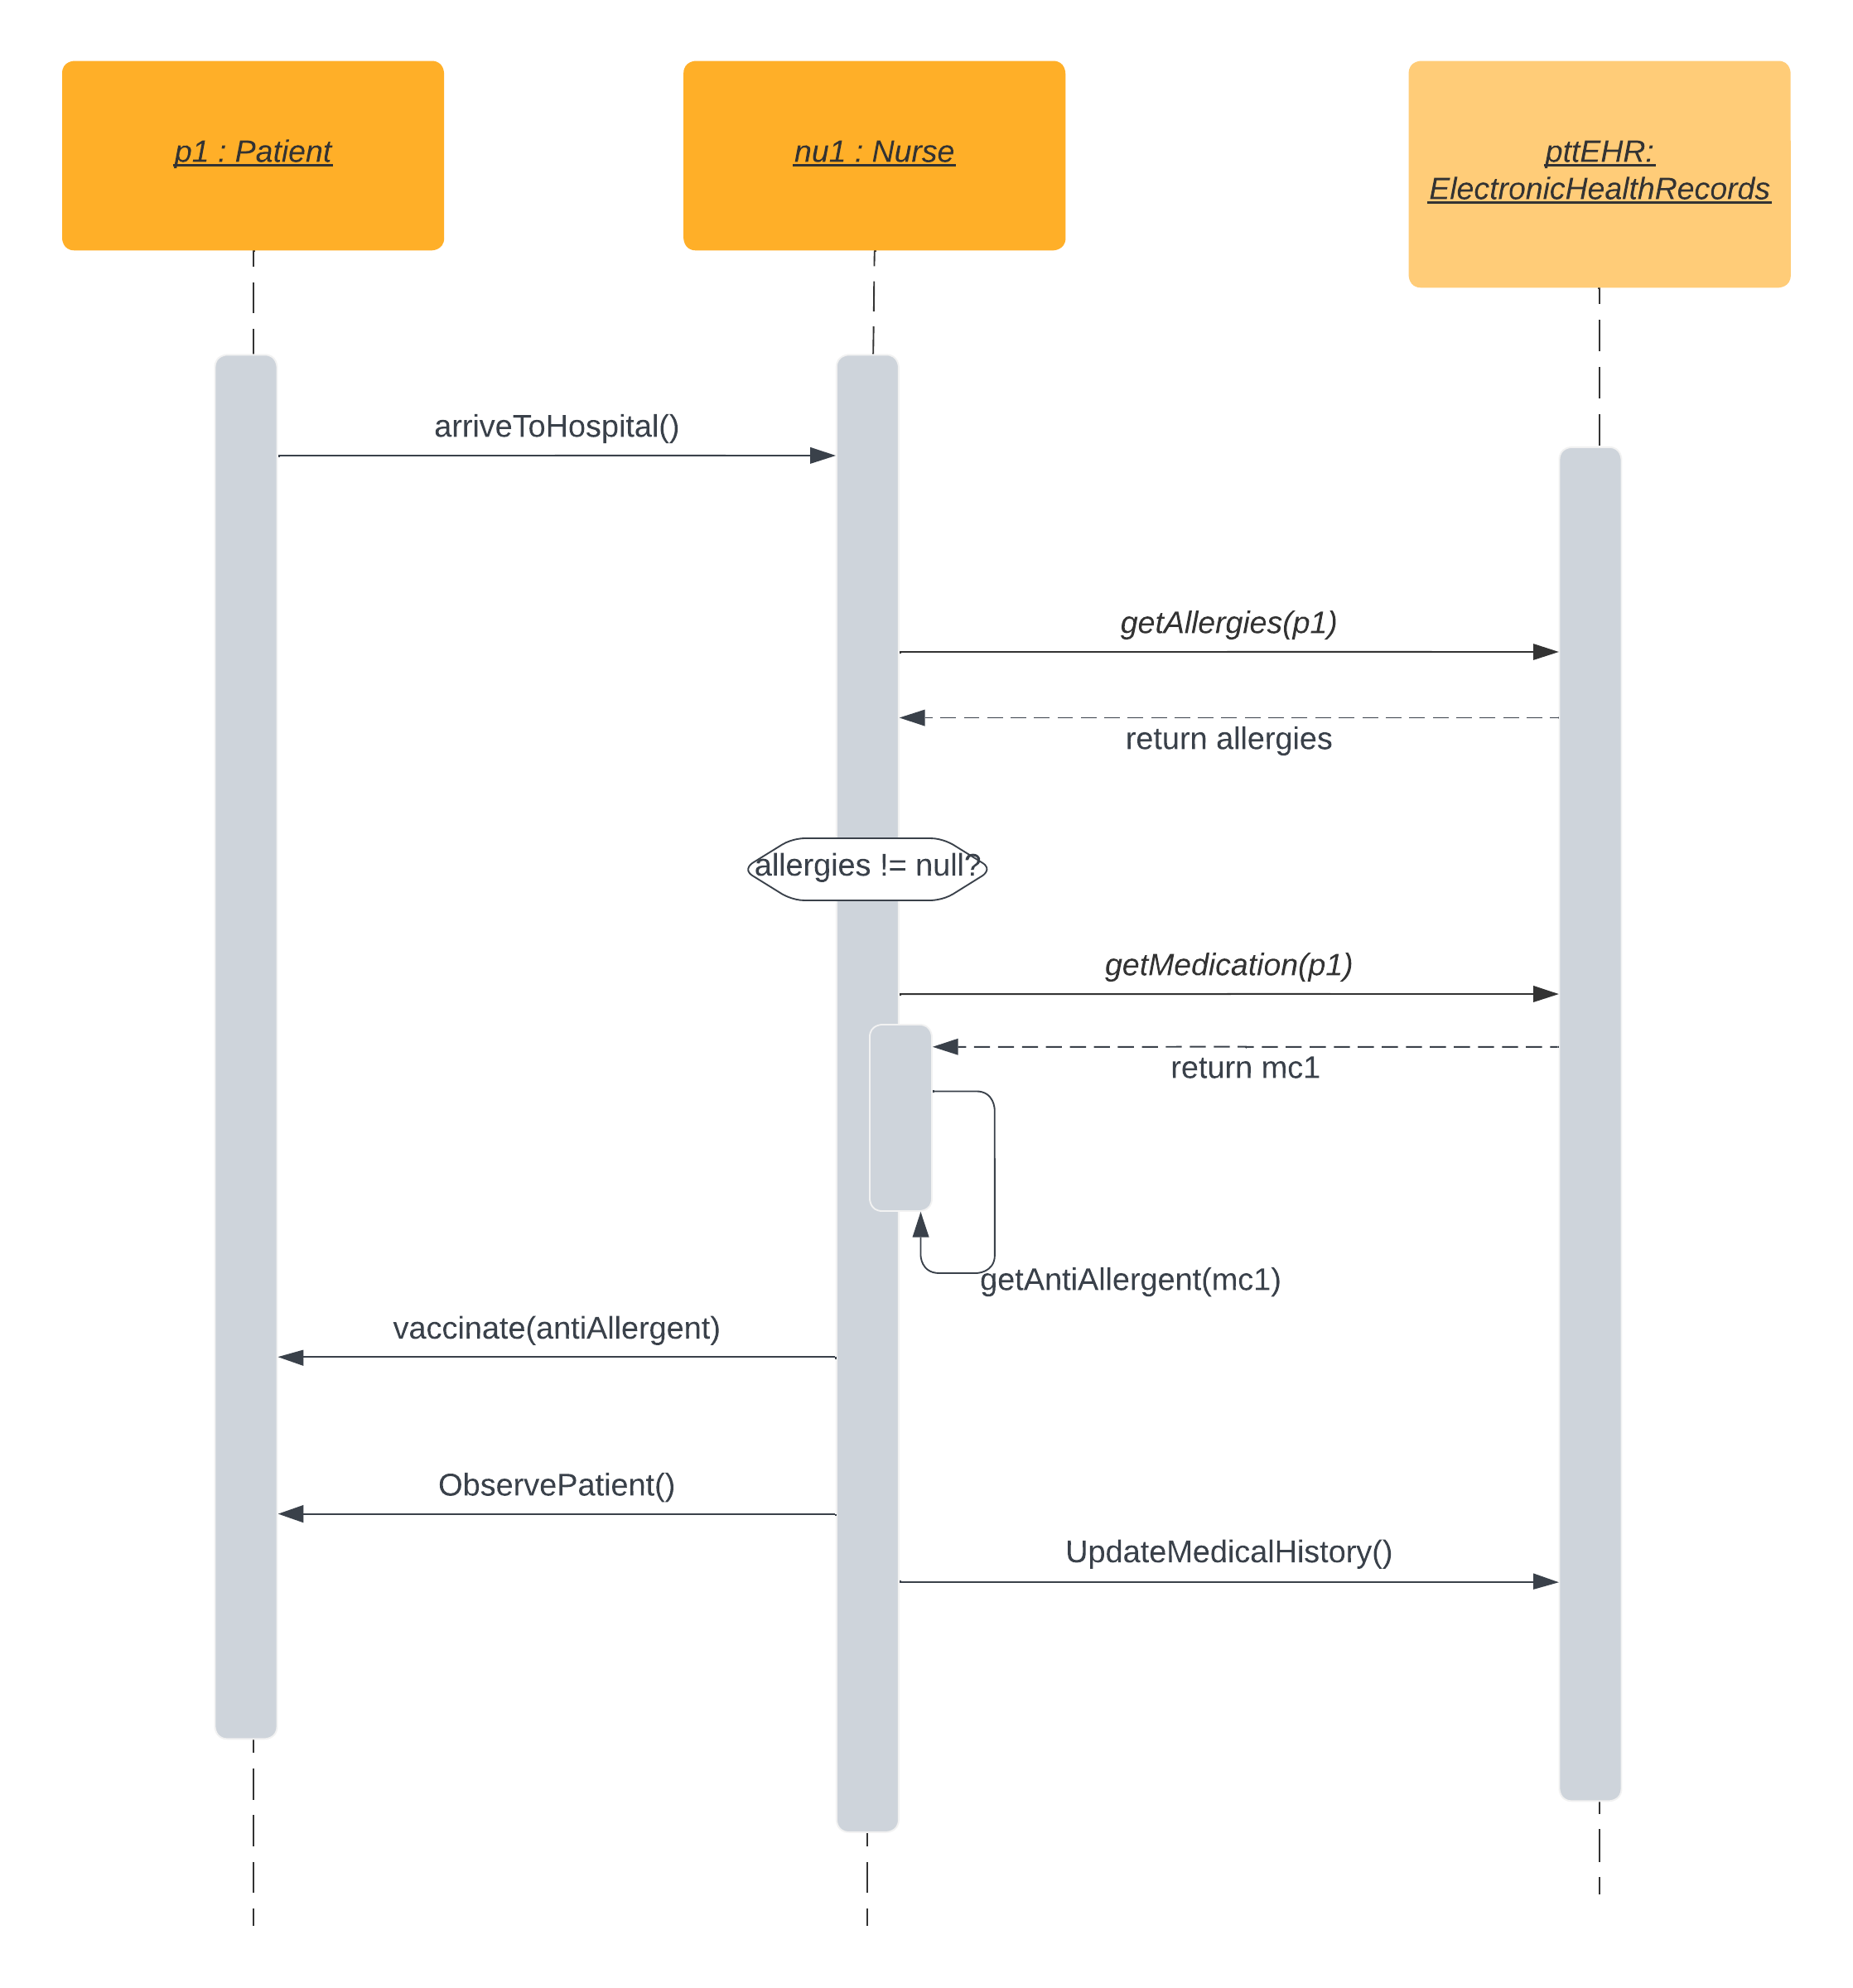
\includegraphics[width=12cm]{src/pic/Vaccination_With_allergies.png}\end{center}
\caption{Visual Sequence Diagram for Vaccination of a Patient with Allergies}
\label{VACA2}
\end{figure}


\section{Use Case Diagram}

\subsection{Reception and Patient UCD}
This use case diagram illustrates the various interactions and functionalities between a receptionist and a patient in the hospital information system.

\textbf{Use Cases}
\begin{itemize}
    \item ScheduleAppointment: This use case allows the receptionist and the patient to schedule an appointment for a specific date and time.
    \item ScheduleHospitalAdmission: The receptionist and the patient can use this use case to schedule a hospital admission for the patient.
    \item PatientRegistration: This use case enables the receptionist and the patient to complete the patient registration process.
    \item PatientHospitalAdmission: The receptionist can initiate the patient's hospital admission process using this use case.
    \item FileMedicalReports: The receptionist can use this use case to file and manage the patient's medical reports.
\end{itemize}

\textbf{Actors}
\begin{itemize}
    \item Receptionist: Represents the hospital receptionist who interacts with the patient and performs administrative tasks.
    \item Patient: Represents the individual seeking medical care from the hospital.
\end{itemize}

\textbf{Relationships}
\begin{itemize}
    \item The Receptionist actor is associated with several use cases, including ScheduleAppointment, ScheduleHospitalAdmission, PatientRegistration, PatientHospitalAdmission, and FileMedicalReports.
    \item The Patient actor is associated with ScheduleAppointment, ScheduleHospitalAdmission, and PatientRegistration.
    \item PatientRegistration extends both ScheduleHospitalAdmission and ScheduleAppointment, indicating that patient registration involves scheduling hospital admissions and appointments.
    \item PatientHospitalAdmission includes PatientRegistration, indicating that the patient's hospital admission process includes patient registration.
    \item NewPatientHospitalAdmission specializes PatientHospitalAdmission, indicating a specific type of patient hospital admission for new patients.
    \item InHospitalPatientAdmission specializes PatientHospitalAdmission, representing the hospital admission process for existing inpatients.
    \item Both NewPatientHospitalAdmission and InHospitalPatientAdmission include BedAllotment, indicating that bed allotment is part of the respective admission processes.
\end{itemize}

\begin{figure}[!htb]
\lstset{language=MontiArc}
\lstinputlisting[
label=lst:recpat,
caption=Use Case Diagram in Moticore UCD] {src/listings/UCD/receptionist_patient.ucd}
\end{figure}


\begin{figure}[!htb]
\begin{center}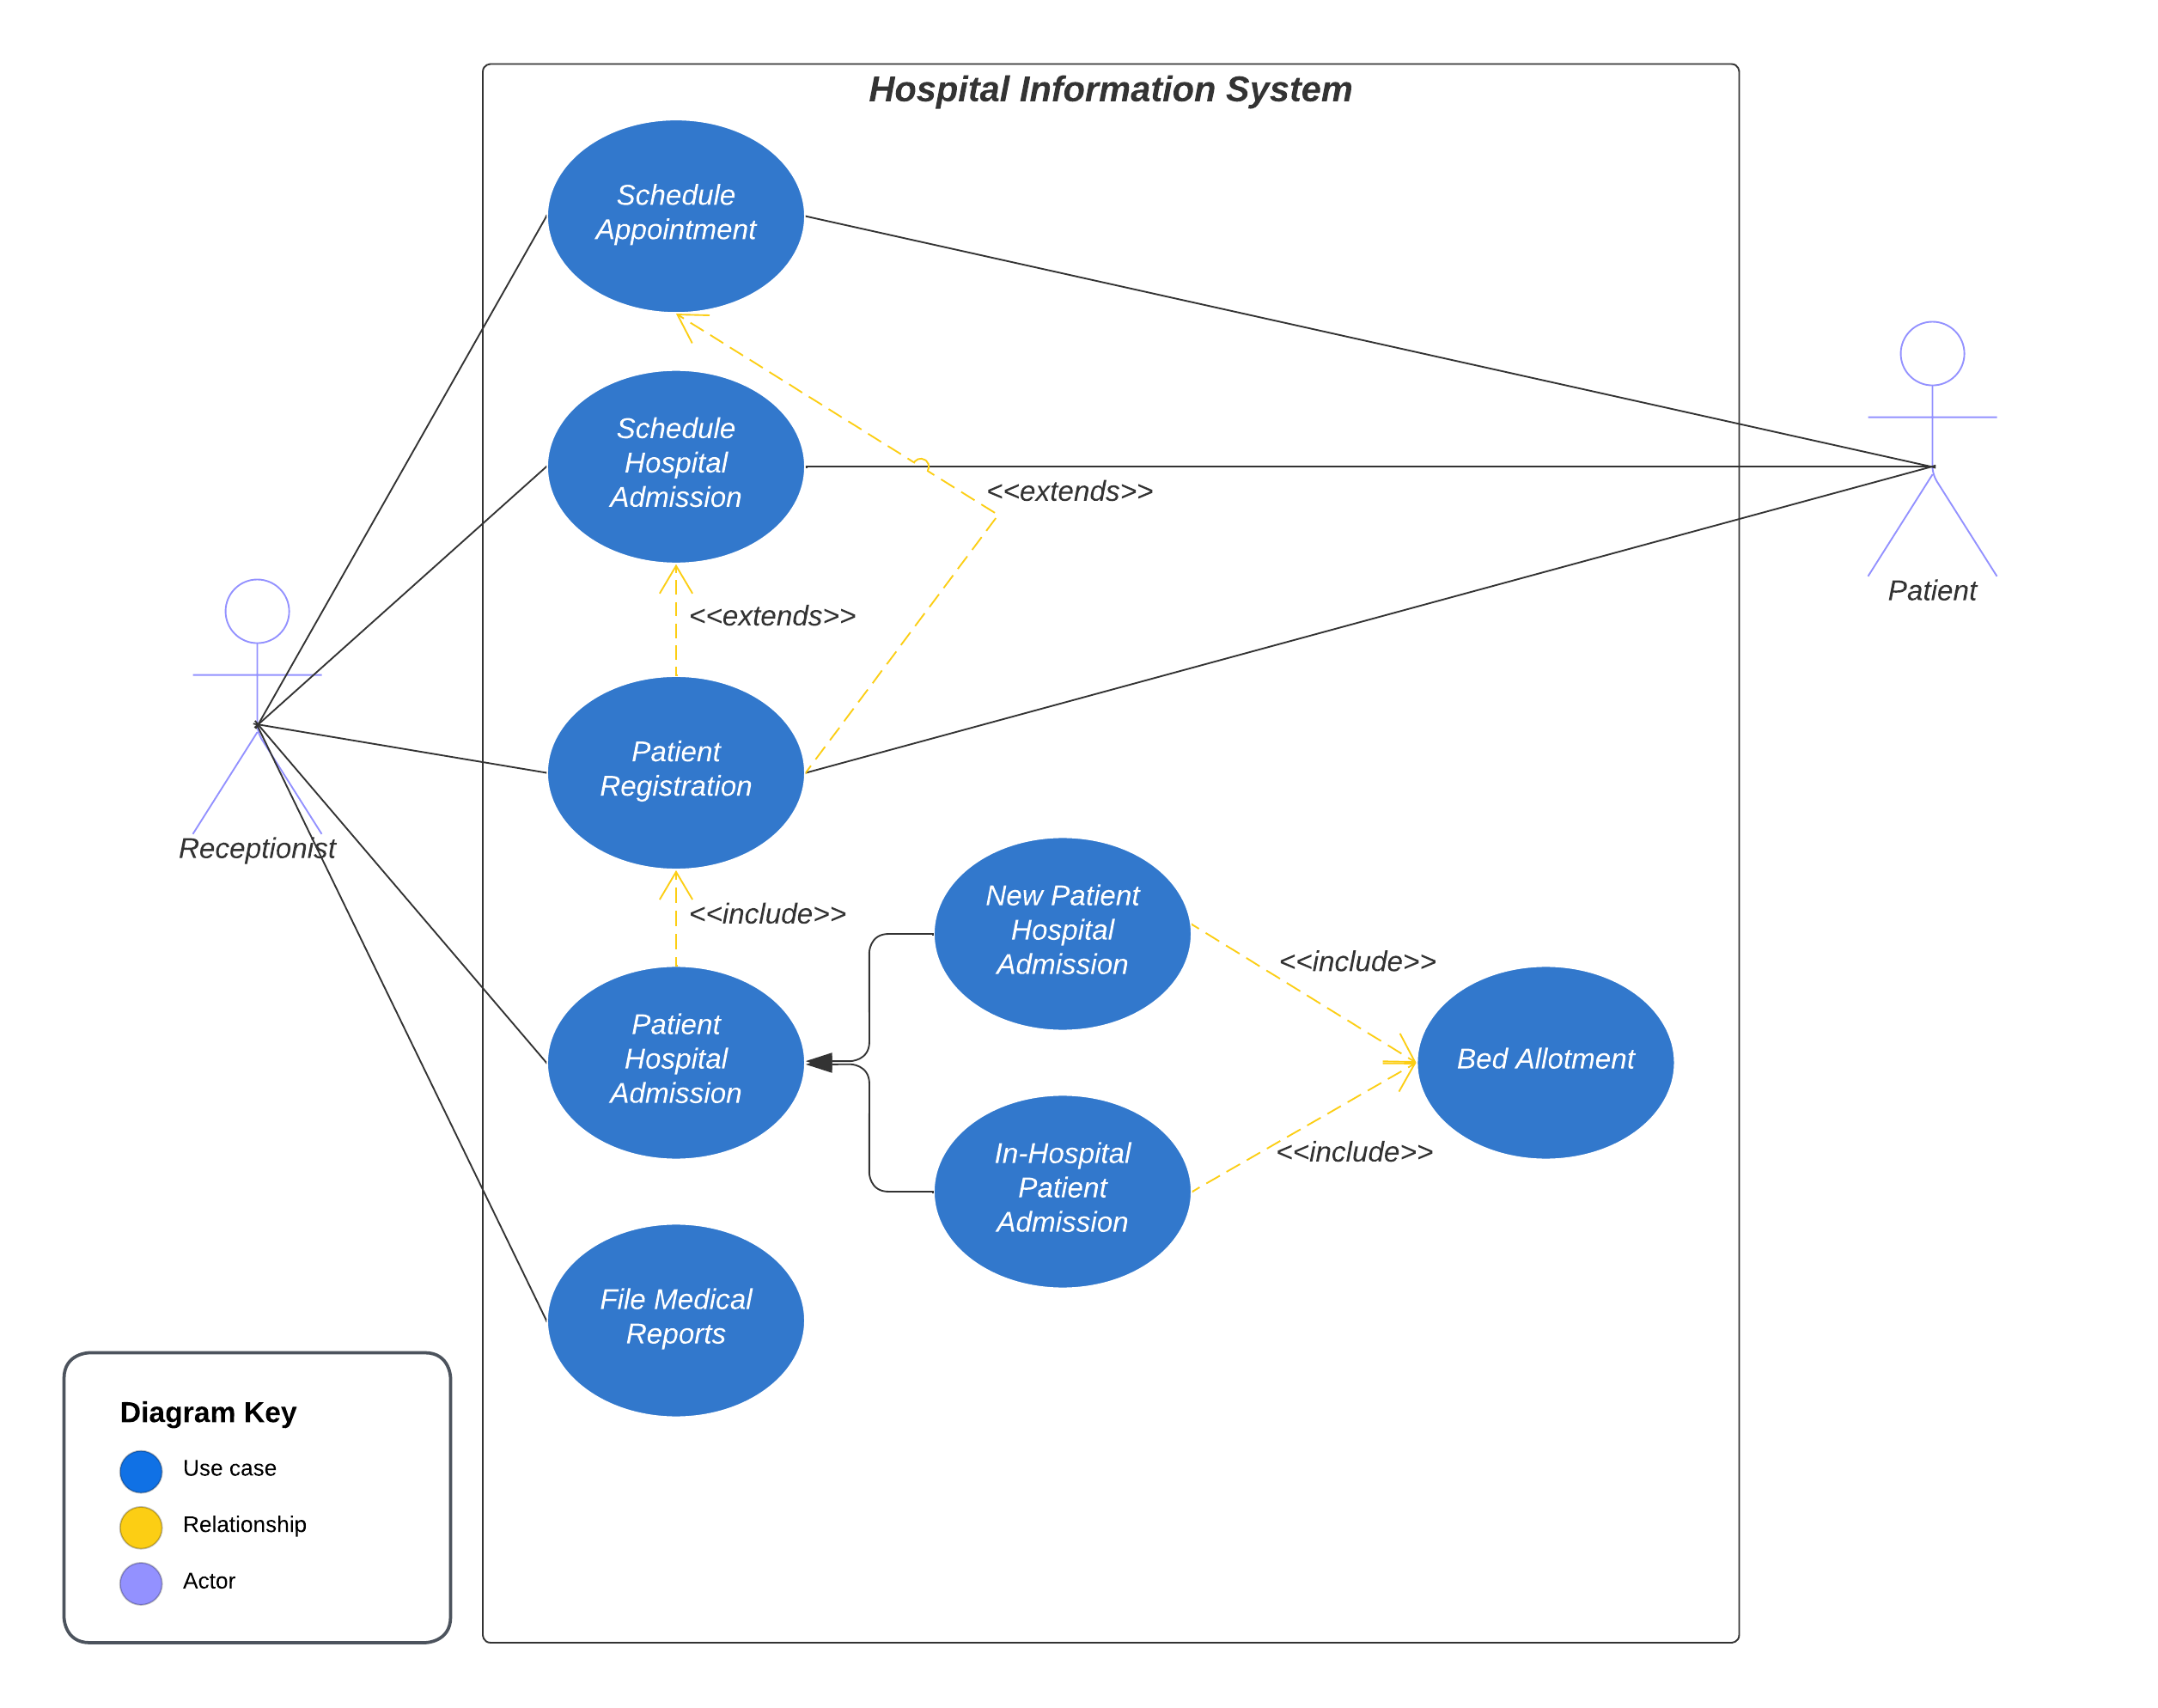
\includegraphics[width=12cm]{src/pic/Diagrams/Receptionist_Patient_UCD.png}\end{center}
\caption{Visual Use Case Diagram of Reception and Patient Case}
\label{RPUCD}
\end{figure}

\subsection{Dischage Patient UCD}

This use case diagram illustrates the interactions and functionalities related to the discharge of a patient from a hospital in the hospital information system.

\textbf{Use Cases}
\begin{itemize}
    \item DischargePatient: Represents the use case where the receptionist performs the patient discharge process.
    \item GenerateBill: This use case extends the ViewEHRs use case and involves generating the patient's bill as part of the discharge process.
\end{itemize}

\textbf{Actors}
\begin{itemize}
    \item Receptionist: Represents the hospital receptionist who is responsible for initiating and managing the discharge process.
\end{itemize}

\textbf{Relationships}
\begin{itemize}
    \item The Receptionist actor is associated with the DischargePatient use case, indicating that the receptionist is responsible for performing the patient discharge process.
    \item GenerateBill extends the ViewEHRs use case, indicating that generating the patient's bill is an additional step within the discharge process.
    \item DischargePatient includes the GenerateBill use case, indicating that generating the bill is a part of the overall discharge process.
    \item DischargeOutPatient specializes the DischargePatient use case, representing the discharge process for patients who were treated as outpatients.
    \item DischargeInPatient specializes the DischargePatient use case, representing the discharge process for patients who were admitted to the hospital as inpatients.
\end{itemize}


\begin{figure}[!htb]
\lstset{language=MontiArc}
\lstinputlisting[
label=lst:dispat,
caption=Use Case Diagram in Moticore UCD for Discharge Patient Use Case] {src/listings/UCD/discharge_patient.ucd}
\end{figure}



\begin{figure}[!htb]
\begin{center}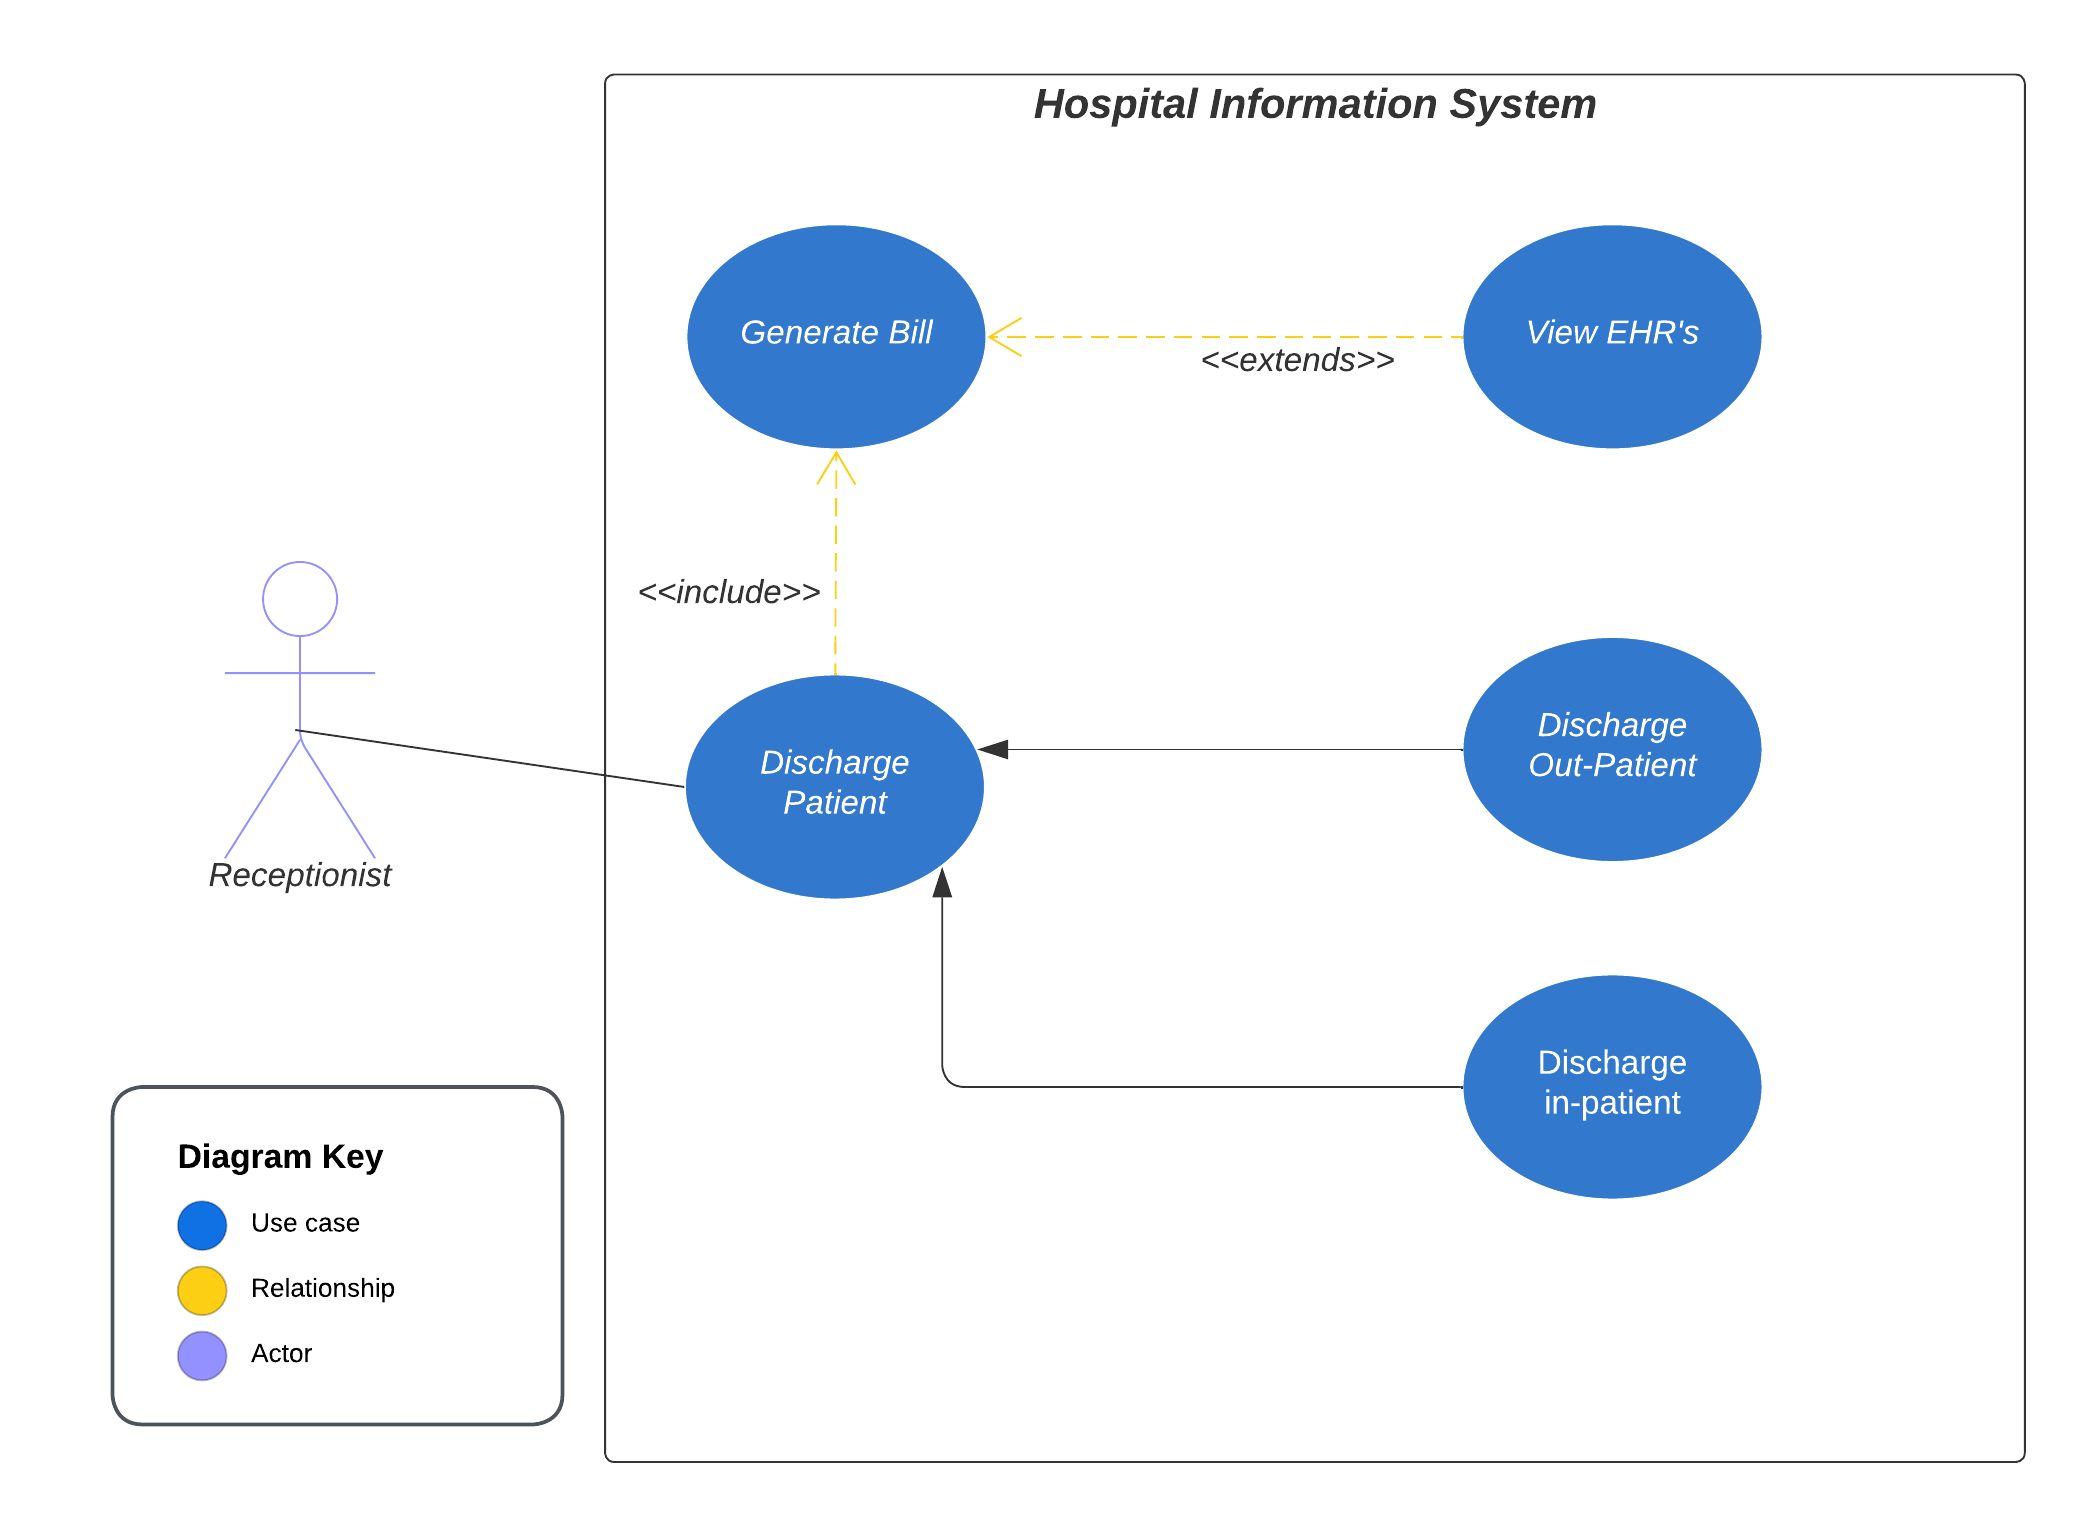
\includegraphics[width=12cm]{src/pic/Diagrams/Dischage_Patient_UCD.png}\end{center}
\caption{Visual Use Case Diagram of Discharge Patient Case}
\label{DPUCD}
\end{figure}


\subsection{Doctor Patient Interaction with EHR Use Case}

This use case diagram illustrates the interactions and functionalities of the Electronic Health Record (EHR) system within the hospital information system. It captures the use cases involving doctors and patients in accessing and managing medical information.

\textbf{Use Cases}
\begin{itemize}
    \item ViewMedicalHistory: This use case allows doctors and patients to view the medical history of the patient.
    \item AddDiagnosis: Doctors can use this use case to add a diagnosis to a patient's medical record.
    \item PrescribeMedication: Doctors can prescribe medication to patients using this use case.
    \item ScheduleAppointment: Patients can schedule an appointment using this use case.
    \item RequestMedication: Patients can request medication through this use case.
    \item ProvideMedicalHistory: Patients can provide their medical history using this use case.
\end{itemize}

\textbf{Actors}
\begin{itemize}
    \item Doctor: Represents the medical professional responsible for diagnosing and treating patients.
    \item Patient: Represents an individual seeking medical care from the hospital.
\end{itemize}

\textbf{Relationships}
\begin{itemize}
    \item The Doctor actor is associated with ViewMedicalHistory, AddDiagnosis, and PrescribeMedication use cases, indicating the functionalities available to doctors.
    \item The Patient actor is associated with ViewMedicalHistory, ScheduleAppointment, RequestMedication, and ProvideMedicalHistory use cases, representing the functionalities accessible to patients.
    \item ViewMedicalHistory extends ProvideMedicalHistory, indicating that the action of viewing the medical history is built upon the patient providing their medical history.
    \item PrescribeMedication includes RequestMedication, indicating that prescribing medication includes the request made by the patient.
\end{itemize}

\begin{figure}[!htb]
\lstset{language=MontiArc}
\lstinputlisting[
label=lst:docpat,
caption=Use Case Diagram in Moticore UCD for Doctor Patient Interaction with EHR Use Case] {src/listings/UCD/doctor_patient.ucd}
\end{figure}



\begin{figure}[!htb]
\begin{center}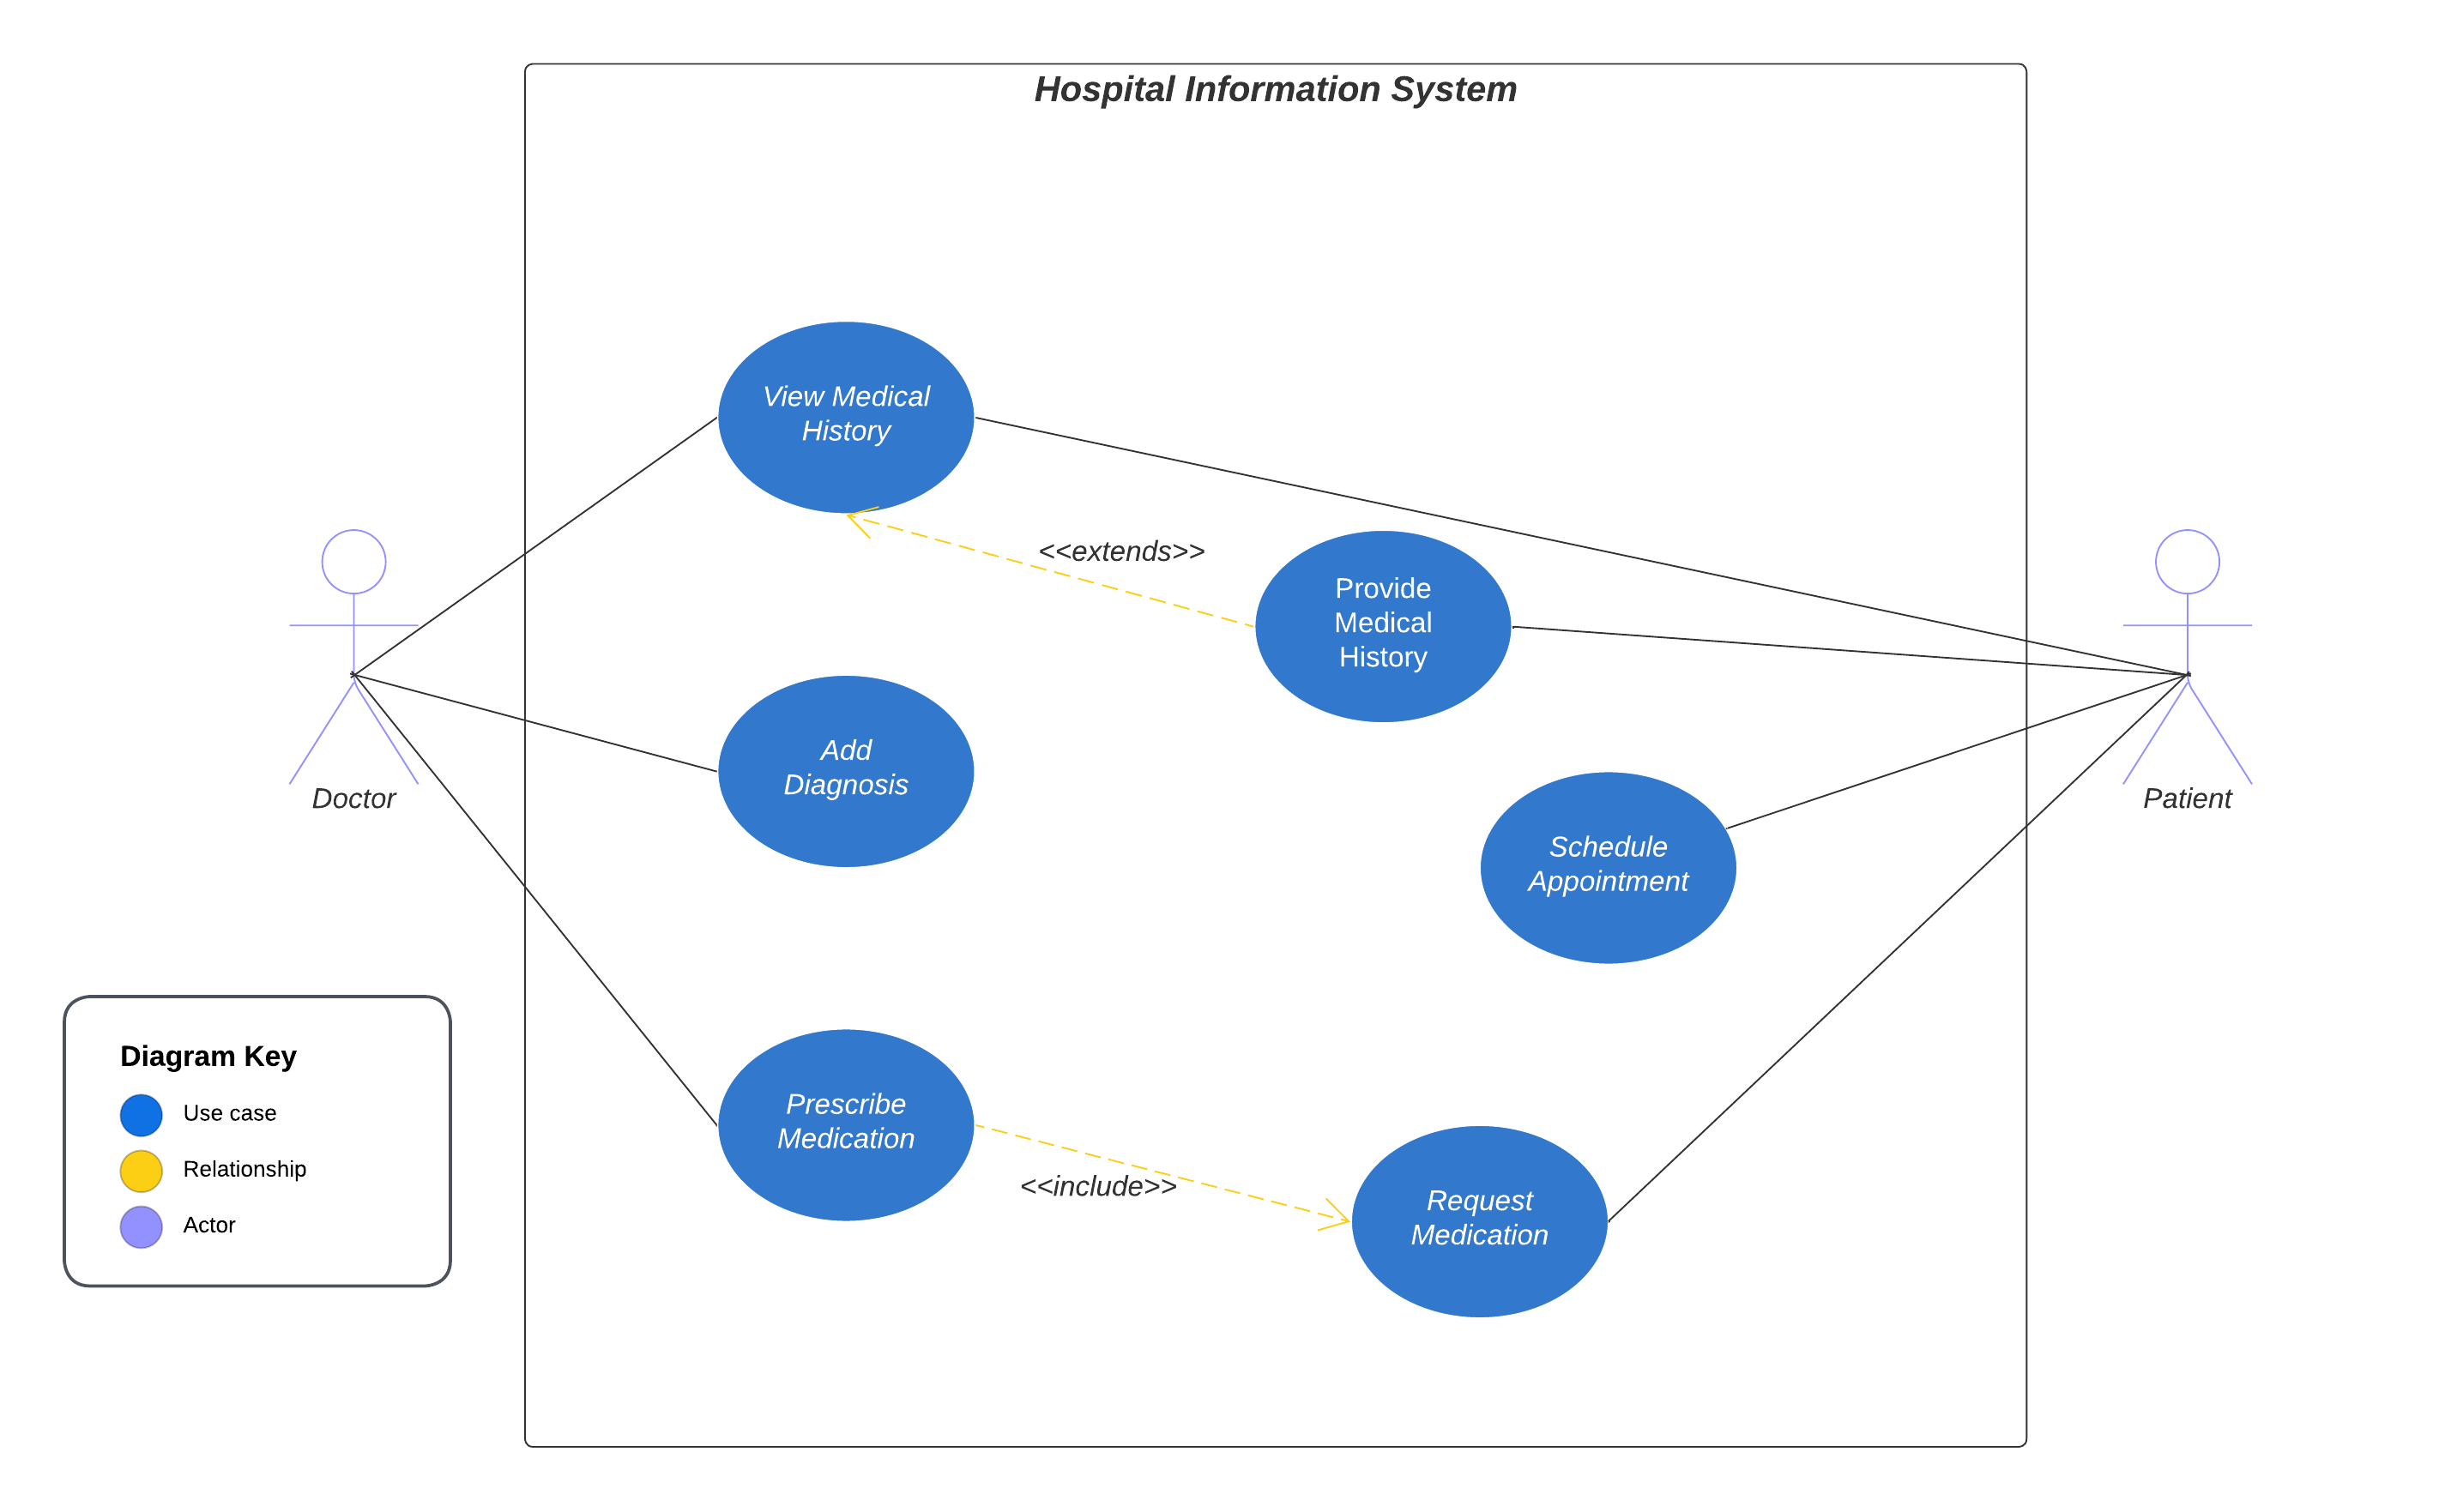
\includegraphics[width=12cm]{src/pic/Diagrams/EHR_Doctor_Patient_UCD.png}\end{center}
\caption{Visual Use Case Diagram of Doctor Patient Interaction with EHR Use Case}
\label{dopaUCD}
\end{figure}

\section{BPMN Diagram}

\begin{figure}[!htb]
\begin{center}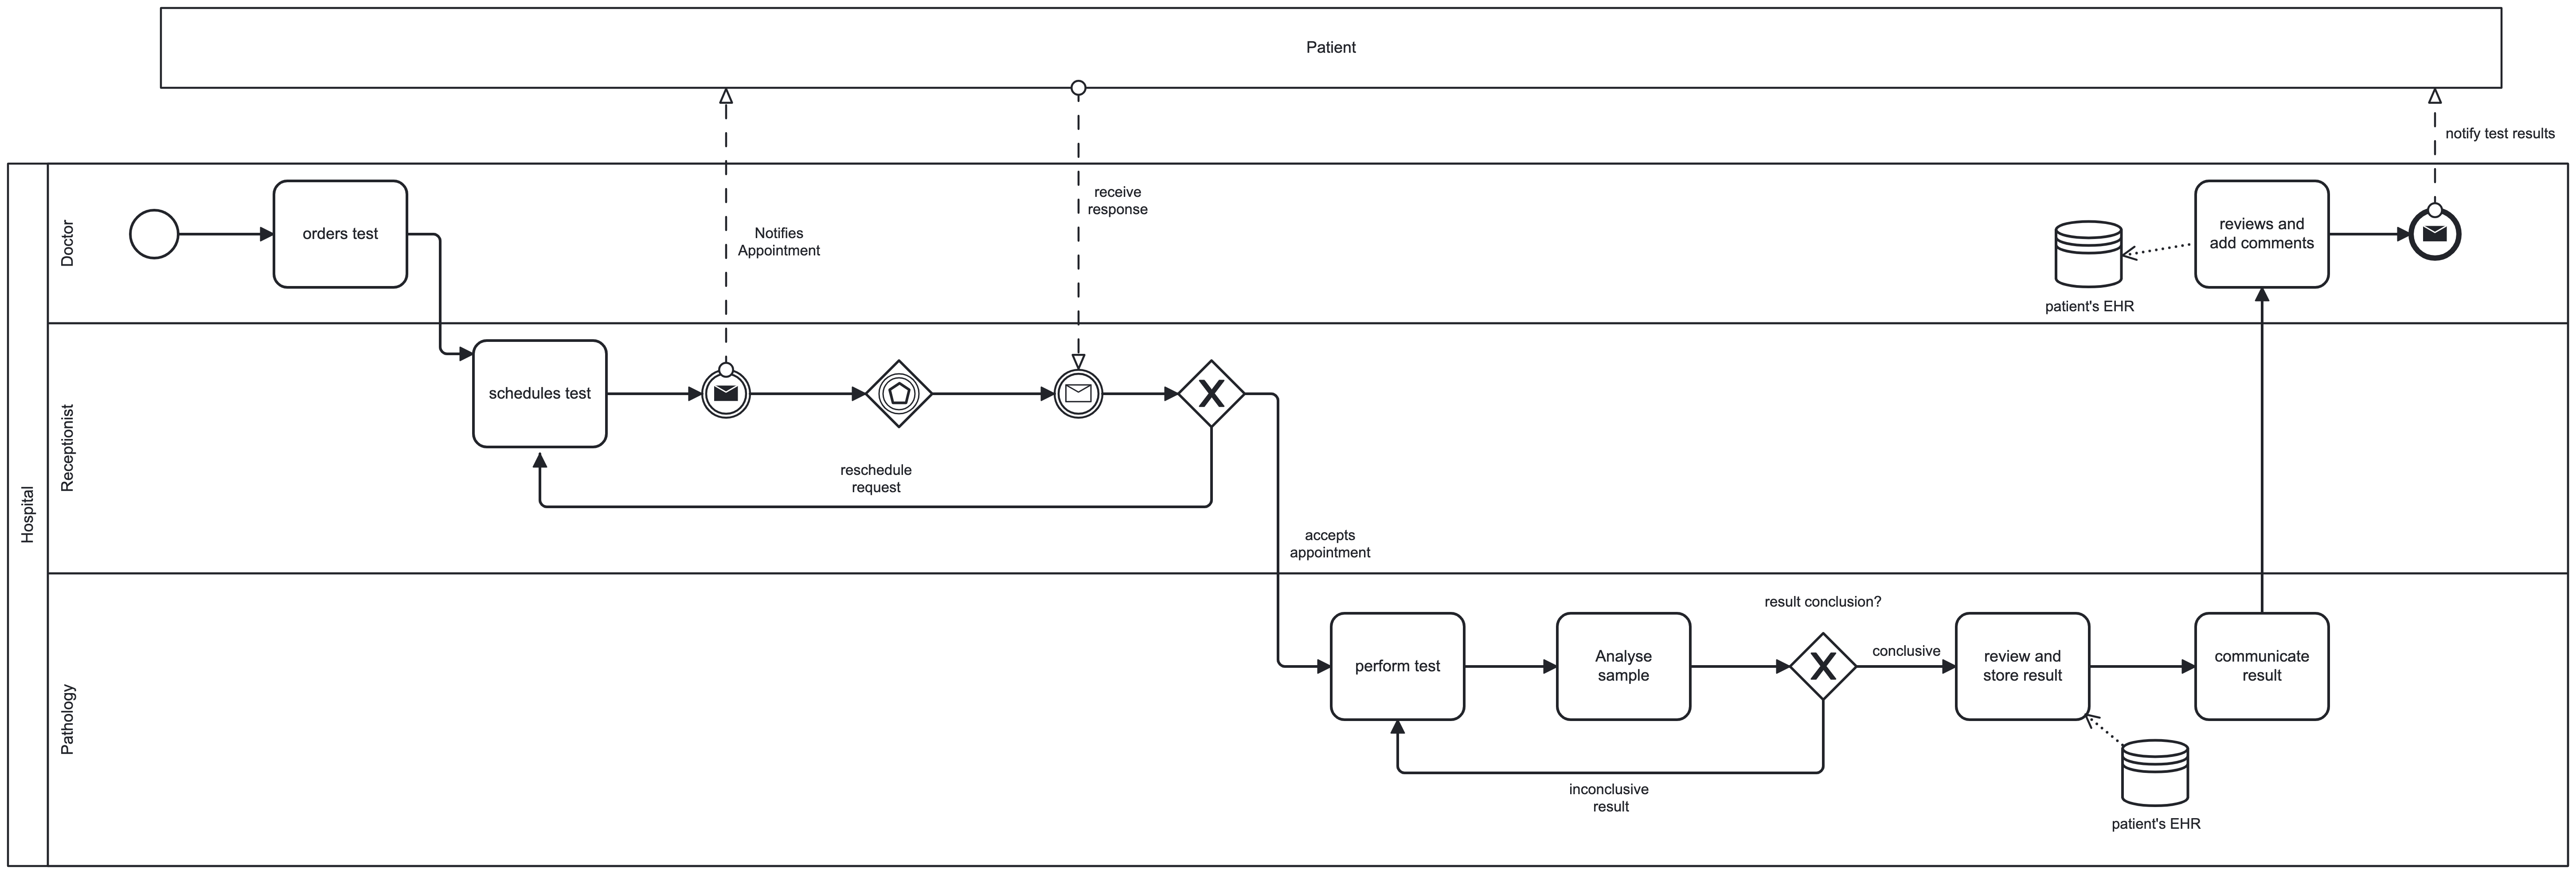
\includegraphics[width=20cm,angle=90]{src/listings/BPMN/lab_bmpn.png}\end{center}
\caption{BPMN Diagram showcasing the process of a doctor scheduling a test}
\label{bpmn}
\end{figure}

In the following BPMN model, the process of a doctor scheduling a test is explained:

\begin{enumerate}
\item The doctor in the hospital orders a test.
\item The receptionist receives the test order and schedules the test.
\item The receptionist notifies the patient about the scheduled appointment.
\item An event-based gateway is used to wait for the patient's response.
\item When the patient responds, it is checked if they want to reschedule the appointment or accept it.
\item If the patient wants to reschedule the appointment, the process loops back to the scheduling step.
\item If the appointment is accepted, the pathologist is assigned to perform the test.
\item The pathologist collects samples for the test and analyzes them.
\item If the test results are inconclusive, the test is performed again.
\item The pathologist repeats the test until the results are conclusive.
\item The conclusive test result is updated in the system and stored under the patient's electronic health record.
\item The test result is communicated to the doctor.
\item The doctor reviews the test result and updates the patient's health record in the health information system.
\item The doctor notifies the patient about the test result.
\end{enumerate}

\let\cleardoublepage\clearpage
